\section{Dataset and Exploratory Data Analysis}
\label{sec:data-eda}

\paragraph{Dataset and data quality.}
We analysed 1,000 English restaurant-review snippets from the public
\texttt{Restaurant\_Reviews.tsv} snapshot
\citep{rajagopal-restaurant-reviews}. The file contains review text
(\texttt{Review}) and a binary sentiment label (\texttt{Liked}, with 0
for negative and 1 for positive), with 500 observations per class.
A row-wise comparison with the UCI Yelp subset \citep{kotzias-sentiment}
found 995 matching text--label pairs after trimming whitespace.
We use the TSV snapshot for all counts below.

We checked for missing fields, blank reviews, unsupported labels,
duplicate text and unusual characters. We applied Unicode NFC
normalization, collapsed whitespace and kept punctuation, accents and
negation. The file contained four reviews with non-ASCII characters,
zero missing or blank fields, and zero flagged control or replacement
characters. Four redundant same-label records were removed before
splitting, and there were zero identical texts with conflicting labels.
The resulting corpus contained 996 distinct reviews, with 497 negative
and 499 positive.

\paragraph{Data partition.}
We used a single stratified 80/20 split with random seed 8017
(Table~\ref{tab:data-eda-split}). The test set contained 100 reviews
per class, and the two partitions shared zero exact review texts after
normalization. Subsequent feature fitting and model selection use the
training partition. The test partition is reserved for final evaluation.

\begin{table}[t]
  \caption{Class counts after deduplication and stratified splitting.}
  \label{tab:data-eda-split}
  \centering
  \begin{tabular}{lrrr}
    \hline
    Partition & Negative & Positive & Total \\
    \hline
    Cleaned & 497 & 499 & 996 \\
    Train & 397 & 399 & 796 \\
    Test & 100 & 100 & 200 \\
    \hline
  \end{tabular}
\end{table}

\paragraph{Review length and vocabulary.}
Negative reviews had a median length of 10 words (interquartile range
6--16), compared with 9 words (6--14) for positive reviews
(Figure~\ref{fig:data-eda-lengths}). The overlapping distributions
suggest that length alone offers limited separation. In the training
set, \emph{not} appeared in 81 of 397 negative reviews (20.4\%).
\emph{Good} appeared in 59 of 399 positive reviews (14.8\%) and 18 of
397 negative reviews (4.5\%). This overlap motivates evaluating
bigrams that can represent local context. We counted each word once per
review for these frequencies and retained negation during stop-word
filtering. The source file has no restaurant or reviewer identifiers,
so the split measures generalization at the review level.

\begin{figure}[t]
  \centering
  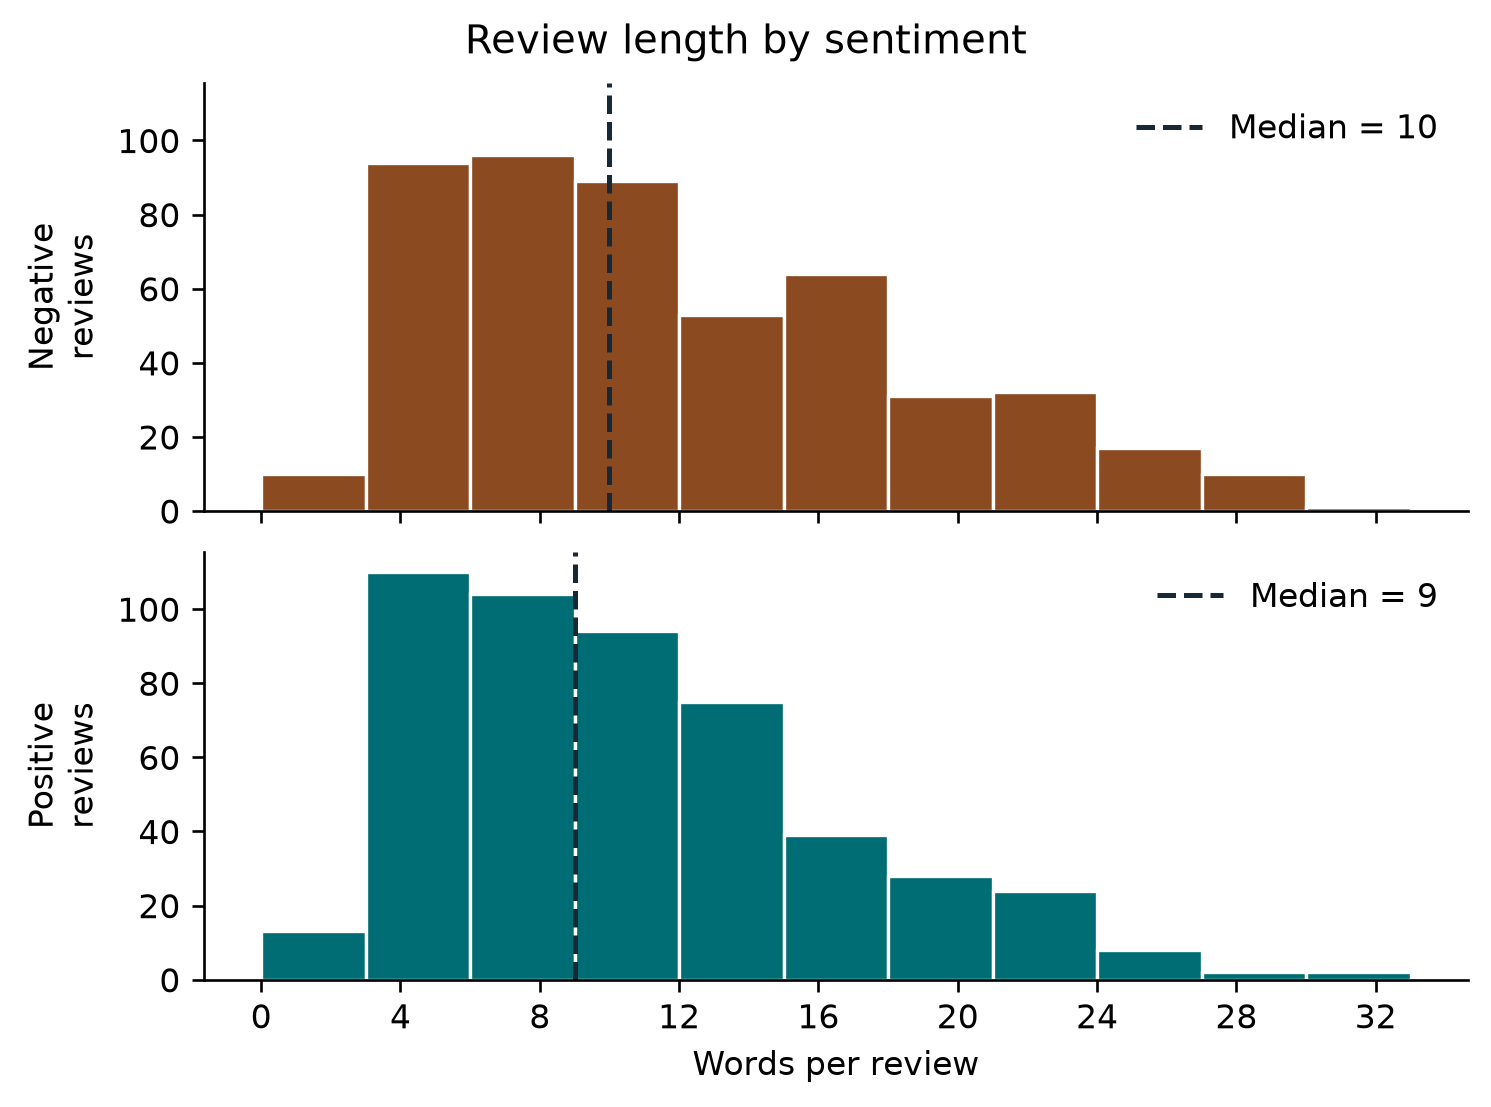
\includegraphics[width=\columnwidth]{../results/figures/eda_review_lengths.png}
  \caption{Word counts in the cleaned corpus by sentiment. The panels
  share histogram bins and axes. Dashed lines mark the class medians.}
  \label{fig:data-eda-lengths}
\end{figure}
